\chapter{Introduction} \label{ch:introduction}

Humankind's push for innovation and problem-solving of the ever extending set of challenges it faces, resulted in a rapid evolution of the technological forefront. 
The development of digital systems capable of processing levels beyond humanly possible, expanded the realm of possibilities in both the scientific and engineering fields.
Applications of this technology, from physics, graphical and meteorological computation, to the now emerging machine learning and deep learning solutions, demand an incredibly high amount of computational resources.

As time passed, resources that were once hardly accessible by end users, due to the elevated cost of acquisition and maintenance, are now made widely available through Cloud Computing.
These circumstances called for a rapid evolution of High Performance Computing (HPC), in the search for performance and power-efficiency optimization. 
The power requirements of HPC centers are increasingly higher, to the point where power supply availability is a main concern in their scaling capabilities. Combined with the growing demand for this technology, it is clear that HPC hardware and software architectures need not only high performance technology solutions, but also power efficient ones.
Deeply heterogeneous systems are capable of achieving the necessary performance per watt levels, due to the exploitation of different hardware components specifically designed with certain applications in mind, i.e. parallel computing.
Aside from power and performance, another relevant quality is predictability, a requirement of video transcoding and medical imaging applications. Predictability acts as a trade-off with respect to power consumption, due to the reservation of higher amounts of computing resources to ensure the satisfaction of requirements. 

The MANGO project was introduced with the objective of enabling the development of user applications on heterogeneous HPC systems.
Initially, the MANGO software portion was developed along with a custom hardware architecture capable of fast reconfiguration, allowing the quick and efficient exploration of manycore architectures for HPC systems.
MANGO focused on what the original developers called the PPP space: power, performance and predictability. 
Citing the initial development goals as stated in \cite{mango_exploring_manycore_architectures}:
\begin{itemize}
    \item Simplify the development of parallel applications accessing heterogeneous hardware platforms.
    \item Enable efficient utilization of the computing resources, with an eye to the application QoS/performance requirements.
    \item Minimize the power consumption of the HPC infrastructure.
\end{itemize}

These objectives can only be achieved through the efficient integration and cooperation of an user-friendly but highly functional programming model, an optimized run-time resource management and a hardware abstraction layer capable of expandability.

\section{Initial software stack}

%TODO tmp diagram
\begin{figure}[ht]
    \centering
    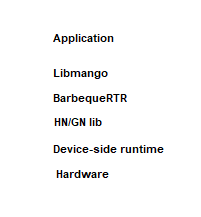
\includegraphics[width=0.5\textwidth]{img/mango-initial-stack.png}
    \captionsetup{justification=centering}
    \caption{MANGO initial software stack}
    \label{fig:mango_initial_stack}
\end{figure}
 
The MANGO software stack, at the beginning of our contribution to the project, looked as shown in figure \ref{fig:mango_initial_stack}.

Starting from the top of the stack, we find the \textbf{Libmango} module, in charge of stablishing the programming model for users of the MANGO system, Libmango exposes an API that provides users with access to the functionalities of the underlying layers. 
It interacts with \textbf{BarbequeRTRM}, the resource manager, responsible for scheduling user applications and allocating system resources according to performance requirements, as well as power and thermal information. BarbequeRTRM also monitors running applications to maintain a complete view of the system, and collect profiling information.

Next in the stack is the Hardware Abstraction Layer, consisting of the \textbf{HN} library and daemon. HN was designed as an abstraction layer for the MANGO custom hardware architecture, supporting PEAK, DCT and nu+ accelerators. To facilitate development and enable running MANGO applications on personal computers, the \textbf{GN} emulator was introduced. The GN library follows the same API as HN, which allows them to be used interchangeably, and emulates the presence of hardware accelerators by using instead the host CPU.
The bottom-most layers are the \textbf{Device Libraries/Drivers}, through which communication with the hardware is stablished and finally the \textbf{Hardware} layer, containing the accelerators themselves.

\section{Thesis Contributions}
\subsection{Python Wrapper}

Our contribution to the MANGO project started with the development of a Python Wrapper of the Libmango module, resulting in a fully functional Python API. Up to that point, only the C and C++ programming languages could be used to interact with the MANGO system, so Python was a perfect fit to expand its compatibility into scripting languages. The project duration was of six months, which also fulfilled the goal of helping us familiarize with the inner workings of the Libmango module. Further details on the Python wrapper implementation are given in the Libmango section of the Architecture chapter \ref{python_wrapper}.

\subsection{JIT Compilation}

As explained in the following chapters, user applications running on the MANGO system consist of a set of tasks (or kernels), that are executed on designated accelerators. 

Previous to our contribution, kernels could only be loaded as binaries (compiled kernels ready for execution). 
Allowing developers to work directly with kernel's source code, instead of requiring pre-compilation, greatly reduces friction in the iterative process of software design.

To achieve this goal, Just In Time compilation of loaded kernels was introduced, enabling developers to load kernels from source code, which are compiled as required by a configurable tool we called the Dynamic Compiler.

The first implementation of the \textbf{Dynamic Compiler} was as an extension of the Libmango module, work that took four months to complete. However, due to a restructuring of the MANGO system, it was later moved to the HHAL module.

\subsection{GPU Support}

The next challenge to tackle was the addition of GPU support to the MANGO system, specifically CUDA compatible Nvidia GPUs. 
With the objective of further fulfilling MANGO's aim at enabling end users to work with highly heterogeneous HPC systems, GPU support is of utmost importance. Apart from their efficient graphics processing capabilities, GPUs are the main accelerator type used in machine learning and deep learning applications due to their highly parallel architecture.

At the time, the HN library played the role of a hardware abstraction layer between hardware-specific libraries and the rest of the MANGO system. Despite being developed with abstraction in mind, the subset of HN-supported hardware accelerators did not merit great levels of generalization, resulting in an abstraction granularity that is too specific for the smooth integration of accelerators such as GPUs.

As a consequence, instead of expanding the HN library, development of the Nvidia Architecture Node (NAN) \ref{NvidiaArchitectureNode}, the platform library in charge of launching kernels on system-available Nvidia devices, begun as an independent MANGO module.

An initial integration effort of the NAN with the Libmango module was successful, enabling kernel execution on target GPUs. 
But a problem with MANGO's structure became increasingly clear. The limited abstraction provided by HN caused the Libmango module to be closely attached to its API and working requirements. This inter-dependency was made evident by the presence of elements like a memory manager in the Libmango module, which was supposed to be architecture agnostic.

A decision was made to restructure the MANGO system with the addition of a new module: HHAL. This module was developed side by side with the NAN.

\subsection{HHAL}

HHAL, which stands for Heterogeneous Hardware Abstraction Layer, was built for the ground up as a solution that enables the easy integration of accelerator architectures to the MANGO system, while freeing Libmango (and other modules) from the inherent complexity of handling multiple architectures. This would also hide the HN library behind the HHAL API.
A detailed explanation of HHAL's implementation is given in section \ref{HHAL}.

While integration of HHAL with the BarbequeRTRM was a smooth process (covered in section \ref{bbque:integration}), Libmango required considerable work.

\subsection{Libmango rework}

For Libmango to fit into the new MANGO structure, a rework of most of its components was necessary. The rework was done with the following conditions and objectives in mind:
\begin{itemize}
    \item Keep the public Libmango API the same, for backwards compatibility.
    \item Remove architecture specific calculations, now carried out by the HHAL module.
    \item Simplify bloated data structures, containing information no longer required.
\end{itemize}

As previously mentioned, the Dynamic Compiler was also moved from Libmango to the HHAL module.

\subsection{Final Software stack}

%TODO tmp diagram (missing drivers layer)
\begin{figure}[ht]
    \centering
    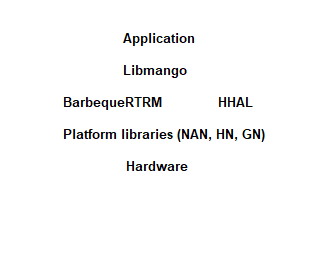
\includegraphics[width=0.5\textwidth]{img/mango-final-stack.png}
    \captionsetup{justification=centering}
    \caption{MANGO final software stack}
    \label{fig:mango_final_stack}
\end{figure}

HHAL and NAN development, Libmango's rework and BarbequeRTRM integration, all took ten months to complete. The implementation work was performed across all modules in an iterative manner, so time dedicated to each module was not measured.
The resulting MANGO software stack can be seen in figure \ref{fig:mango_final_stack}.

\section{Document Structure}

The document is structured as follows:

First, in chapter \ref{ch:StateOfTheArt}, we present a detailed study of the State of the Art, regarding relevant technologies and their evolution through time. We also expand upon the gaps left by covered technologies, and MANGO's role in closing them.

A thorough Architecture Description is given in chapter \ref{ch:ArchitectureDescription}, going over each module of the MANGO software stack.

In chapter \ref{ch:ExperimentalResults}, Experimental Results and explanations of each of the conducted experiments are described.

Finally, in chapter \ref{ch:Conclusions}, we draw the final conclusions, and talk about future work that may be carried out.


